\documentclass{homework}
\usepackage{ctex, bm}
\usepackage[ruled,vlined]{algorithm2e}
\usepackage{booktabs}
\usepackage{multirow}
\usepackage{siunitx}
\usepackage{graphicx}
% \usepackage{subcaption}
\usepackage{caption}
\author{李健宁}
\class{机器学习中的优化问题}
\date{\today}
\title{Homework 8}
% \address{Bayt El-Hikmah}

\graphicspath{{./media/}}

\begin{document} \maketitle

\question

\begin{sol}
    \subsection*{1. Backtracking 停止条件}

backtracking line search 终止条件为:
\[f(\bm{x} + t \Delta \bm{x}) \leq f(\bm{x}) + \alpha t \nabla f(\bm{x})^T \Delta \bm{x},\]
其中常数 \( \alpha \in (0, \frac{1}{2}) \)。

我们利用函数在点 \( \bm{x} \) 处的二阶泰勒展开:
\[f(\bm{x} + t \Delta \bm{x}) = f(\bm{x}) + t \nabla f(\bm{x})^T \Delta \bm{x} + \frac{1}{2} t^2 \Delta \bm{x}^T \nabla^2 f(\bm{\xi}) \Delta \bm{x},\]
其中 \( \bm{\xi} \) 是位于 \( \bm{x} \) 与 \( \bm{x} + t \Delta \bm{x} \) 之间的某个点。

因为 \( \nabla^2 f(\bm{\xi}) \preceq M \bm{I} \),因此
\begin{equation}\label{quad}
    f(\bm{x} + t \Delta \bm{x}) \leq f(\bm{x}) + t \nabla f(\bm{x})^T \Delta \bm{x} + \frac{1}{2} M t^2 \|\Delta \bm{x}\|^2.
\end{equation}

当\(t \leq \frac{-\nabla f(\bm{x})^T \Delta \bm{x}}{M \|\Delta \bm{x}\|^2}\)时,因为\( \alpha \in (0, \frac{1}{2}) \),所以\(t \leq \frac{-2 (1 - \alpha) \nabla f(\bm{x})^T \Delta \bm{x}}{M \|\Delta \bm{x}\|^2}.\)
代入(\ref{quad}),有
\begin{align*}
f(\bm{x} + t \Delta \bm{x}) \leq &f(\bm{x}) + t (\nabla f(\bm{x})^T \Delta \bm{x} + \frac{1}{2} M t \|\Delta \bm{x}\|^2)\\
\leq& f(\bm{x}) +  t (\nabla f(\bm{x})^T \Delta \bm{x} - (1-\alpha)\nabla f(\bm{x})^T \Delta \bm{x})\\
= & f(\bm{x}) +  \alpha t \nabla f(\bm{x})^T \Delta \bm{x},
\end{align*}

\subsection*{2. Backtracking 迭代次数上界}

假设初始步长为 \( t_0 \),每次回溯将当前步长乘以 \( \beta \in (0, 1) \),第 \( k \) 次回溯后的步长为\(t_k = \beta^k t_0.\)

迭代停止时有
\[
t_k= \beta^k t_0 \leq \frac{-\nabla f(\bm{x})^T \Delta \bm{x}}{M \|\Delta \bm{x}\|^2}.
\]

解不等式得
\[
k \leq \left\lceil \log_{1/\beta} \left( \frac{M t_0 \|\Delta \bm{x}\|^2}{- \nabla f(\bm{x})^T \Delta \bm{x}} \right) \right\rceil.
\]
\end{sol}

\question

\begin{sol}

定义函数 \(\phi(\alpha) = f(\mathbf{x}^{(k)} + \alpha \mathbf{d}^{(k)})\),则 \(\alpha_k\) 是 \(\phi(\alpha)\) 的极小点,因此\(\phi'(\alpha_k) = 0.\)
根据链式法则,
\[\phi'(\alpha) = \nabla f(\mathbf{x}^{(k)} + \alpha \mathbf{d}^{(k)})^T \cdot \mathbf{d}^{(k)},\]
代入 \(\alpha_k\),得到
\[\nabla f(\mathbf{x}^{(k+1)})^T \cdot \mathbf{d}^{(k)} = 0.\]

由于 \(\mathbf{x}^{(k+1)} - \mathbf{x}^{(k)} = \alpha_k \mathbf{d}^{(k)}\),可得
\[\nabla f(\mathbf{x}^{(k+1)})^T \cdot (\mathbf{x}^{(k+1)} - \mathbf{x}^{(k)}) 
= \alpha_k \nabla f(\mathbf{x}^{(k+1)})^T \cdot \mathbf{d}^{(k)} = 0.\]

所以
\[\mathbf{x}^{(k+1)} - \mathbf{x}^{(k)} \perp \nabla f(\mathbf{x}^{(k+1)}).\]
\end{sol}

\question

\begin{sol}
    针对$\alpha = 0.1, \beta = 0.3$给出$\log(f(x)-p^*)$和步长随迭代次数的变化。    
\begin{figure}[h]
    \centering
    \begin{minipage}[t]{0.48\textwidth}
        \centering
        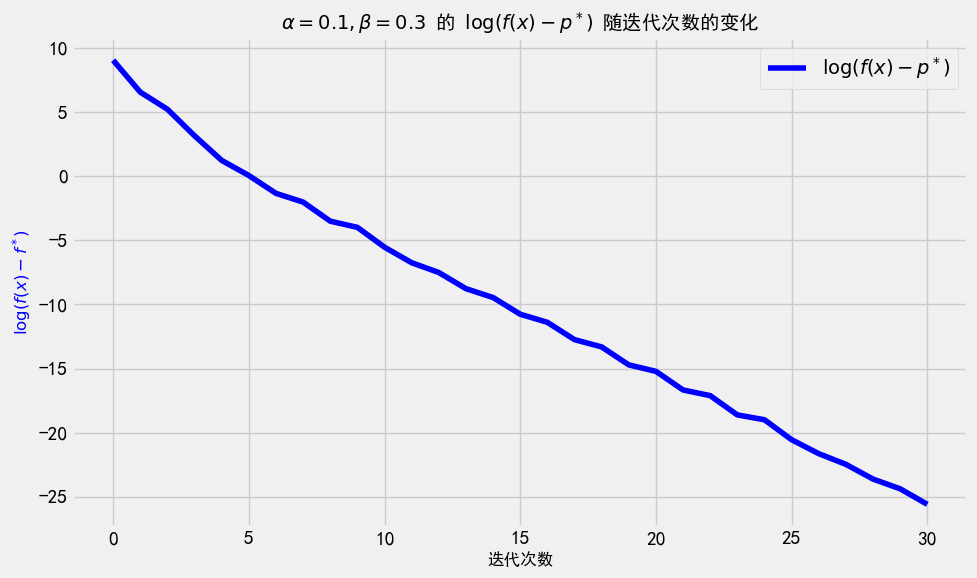
\includegraphics[width=\linewidth]{3-1.png}
        \caption{$\alpha=0.1, \beta=0.3$ 的 $\log(f(x) - p^*)$ 随迭代次数的变化}
        % \label{fig:enter-label}
    \end{minipage}
    \hfill % 添加一些水平间距
    \begin{minipage}[t]{0.48\textwidth}
        \centering
        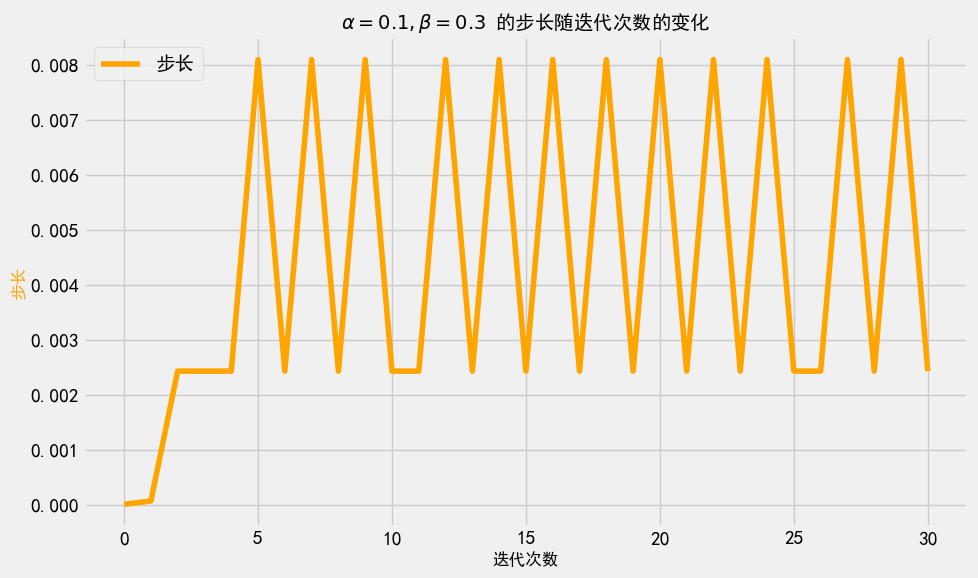
\includegraphics[width=\linewidth]{3-2.png}
        \caption{$\alpha=0.1, \beta=0.3$ 的步长随迭代次数的变化}
    \end{minipage}
\end{figure}


我们选取了$\alpha\in [0.01, 0.1, 0.3, 0.49], \beta\in[0.1, 0.2, 0.3, 0.4, 0.5, 0.6, 0.7, 0.8, 0.9]$绘制迭代次数和参数的关系。实验中,我们选取的停止标准是$\nabla f(x) \le \eta = 10^{-4}$,迭代次数上限是$1000$次。

\begin{figure}[h]
    \centering
    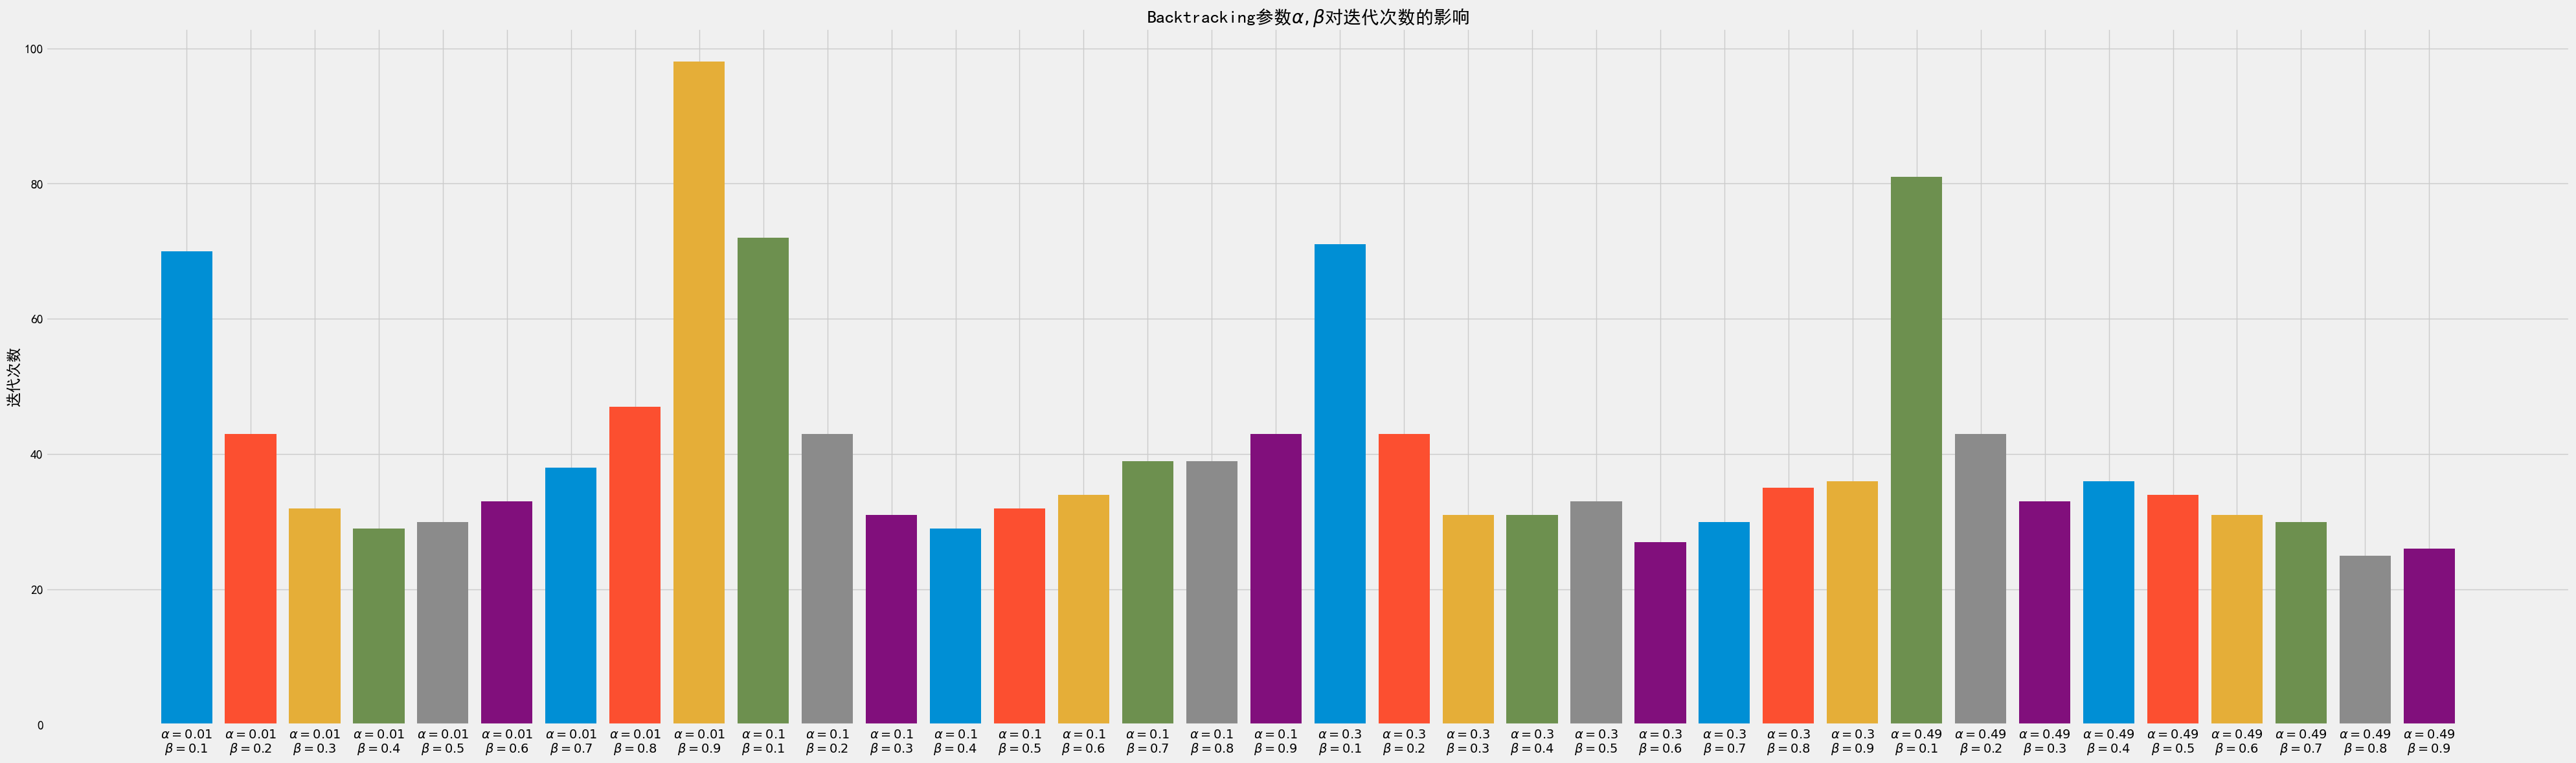
\includegraphics[width=1\linewidth]{3-3.png}
    \caption{Backtracking参数$\alpha, \beta$对迭代次数的影响\protect\footnote{我们省略了超过迭代次数上限($1000$)的参数和相应的迭代次数。}}
\end{figure}
\begin{figure}[h]
    \centering
    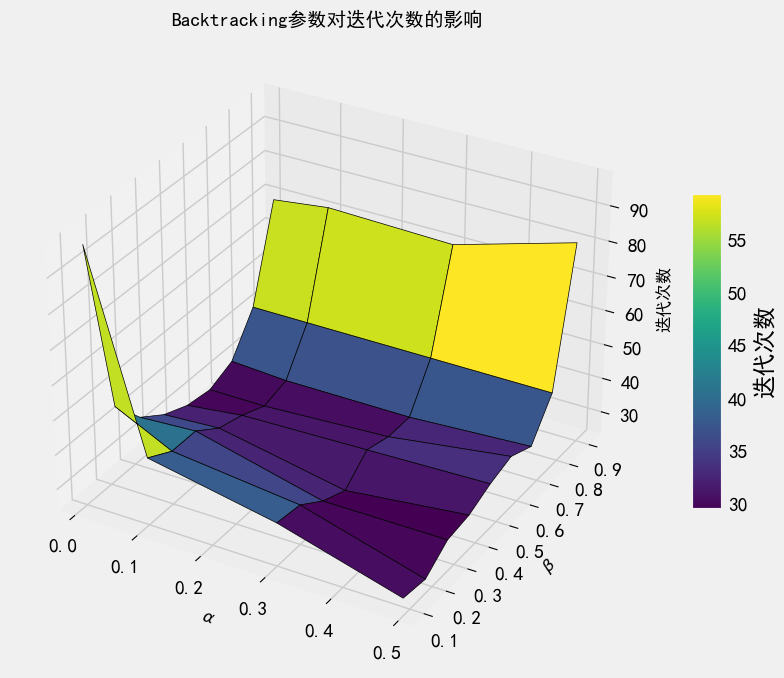
\includegraphics[width=0.5\linewidth]{3-4.png}
    \caption{Backtracking参数$\alpha, \beta$对迭代次数的影响}
\end{figure}


能够发现,$\nabla f(x) \le \eta = 10^{-4}$的停止标准相对来说比较严苛。Backtracking参数选取上,更加接近$0.5$的$\beta$和$\alpha$收敛更快。在$\beta$较小时,$\alpha$的选择对收敛行为影响较大,其他情况则主要依赖于$\beta$,但迭代次数变化的范围整体来看较小。

\end{sol}

\question 

\begin{sol}
    先给出伪代码。
    
    \begin{algorithm}[H]
\caption{Steepest Descent in $\ell_\infty$-norm}
\KwIn{Objective function $f(x)$, gradient $\nabla f(x)$, initial point $x_0$, tolerance $\eta$, backtracking parameters $\alpha$, $\beta$}
\KwOut{Approximate minimizer $x$}
$x \leftarrow x_0$\;
\Repeat{$\|g\|_2 \leq \eta$}{
    $g \leftarrow \nabla f(x)$\;
    $d \leftarrow -\operatorname{sign}(g)$\;
    $t \leftarrow 1$\;
    \While{$f(x + t d) > f(x) + \alpha t g^T d$}{
        $t \leftarrow \beta t$\;
    }
    $x \leftarrow x + t d$\;
}
\end{algorithm}

类似上一题,针对$\alpha = 0.1, \beta = 0.1$给出$\log(f(x)-p^*)$和步长随迭代次数的变化。
\begin{figure}[h]
    \centering
    \begin{minipage}[t]{0.48\textwidth}
        \centering
        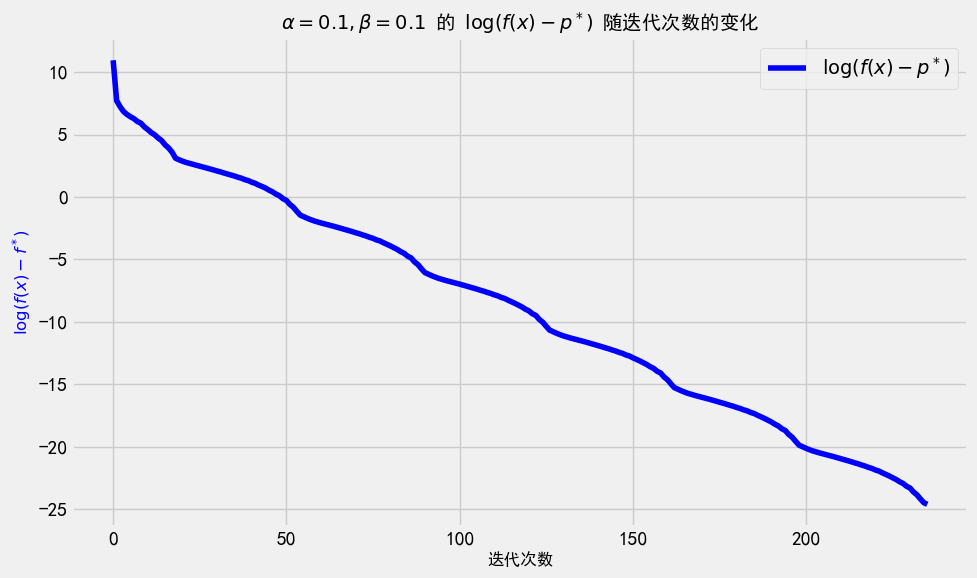
\includegraphics[width=\linewidth]{4-1.png}
        \caption{$\alpha=0.1, \beta=0.1$ 的 $\log(f(x) - p^*)$ 随迭代次数的变化}
        % \label{fig:enter-label}
    \end{minipage}
    \hfill % 添加一些水平间距
    \begin{minipage}[t]{0.48\textwidth}
        \centering
        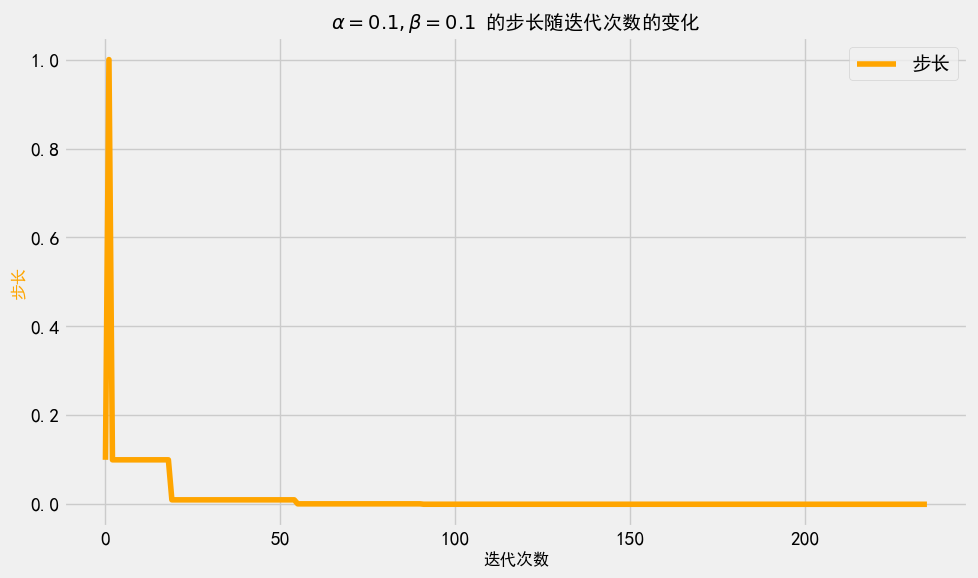
\includegraphics[width=\linewidth]{4-2.png}
        \caption{$\alpha=0.1, \beta=0.1$ 的步长随迭代次数的变化}
    \end{minipage}
\end{figure}

我们选取了$\alpha\in [0.01, 0.1, 0.3, 0.49], \beta\in[0.1, 0.2, 0.3, 0.4, 0.5, 0.6, 0.7, 0.8, 0.9]$绘制迭代次数和参数的关系。实验中,我们选取的停止标准是$\nabla f(x) \le \eta = 10^{-4}$,迭代次数上限是$1000$次。
\begin{figure}[h]
    \centering
    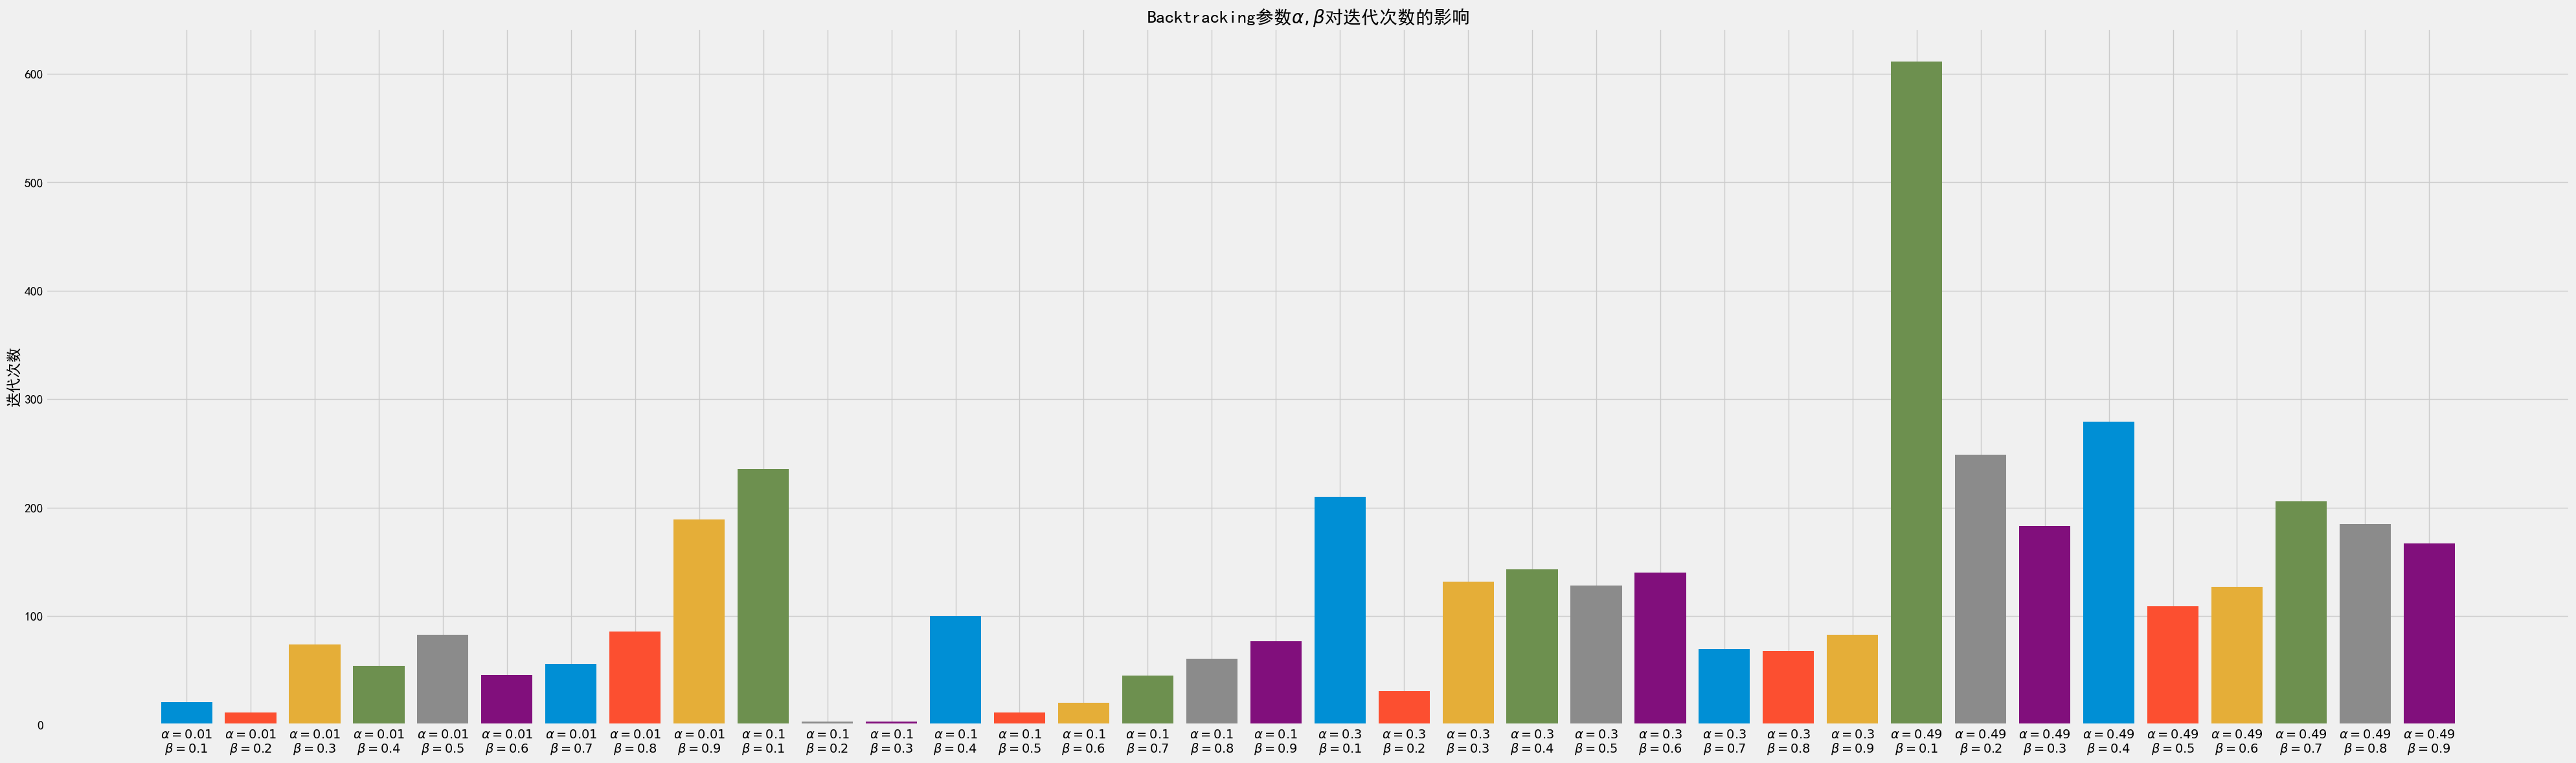
\includegraphics[width=1\linewidth]{4-3.png}
    \caption{Backtracking参数$\alpha, \beta$对迭代次数的影响\protect\footnote{我们省略了超过迭代次数上限($1000$)的参数和相应的迭代次数。}}
\end{figure}
\begin{figure}[h]
    \centering
    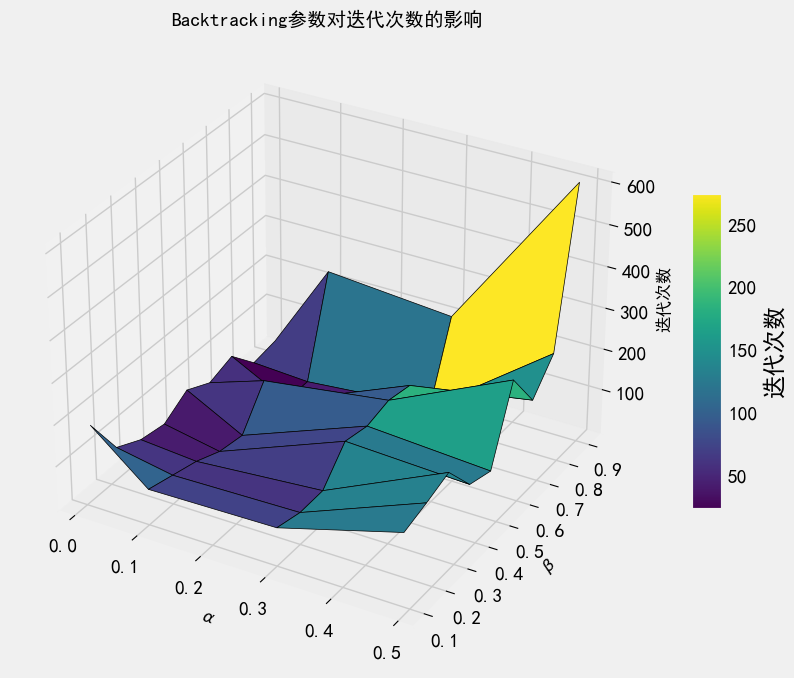
\includegraphics[width=0.5\linewidth]{4-4.png}
    \caption{Backtracking参数$\alpha, \beta$对迭代次数的影响}
\end{figure}

能够发现,$\nabla f(x) \le \eta = 10^{-4}$的停止标准相对来说依旧比较严苛。Backtracking参数选取上,较小的$\alpha$和$\beta$收敛更快。在$\beta$较大时,$\alpha$的选择对收敛行为影响较大,其他情况迭代次数的整体波动不大。

\end{sol}

\question 

\begin{sol}

根据题意,我们分别采取Damped Newton法和Gauss Newton法求解优化问题,并展示求解结果。在Damped Newton法中,我们需要选择Backtracking的参数,这里选择的参数是$\alpha = 0.3, \beta= 0.5$,根据课本中的典型参数值,同时希望能够较快收敛。(事实上,选取更小的$\beta$能够(在时间上)更快收敛。)根据结果(图\ref{5}、\ref{5-2}),Gauss Newton法在解决非线性最小平方问题上确实表现上佳。

\begin{figure}[h]
    \centering
    \begin{minipage}[t]{0.48\textwidth}
        \centering
        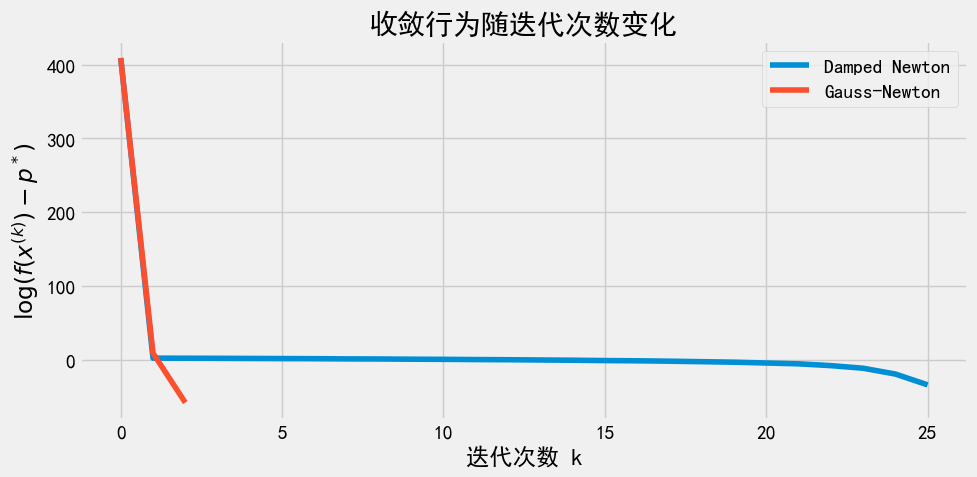
\includegraphics[width=\linewidth]{5-1.png}
        \caption{收敛行为随迭代次数变化}\label{5}
    \end{minipage}
    \hfill % 添加一些水平间距
    \begin{minipage}[t]{0.48\textwidth}
        \centering
        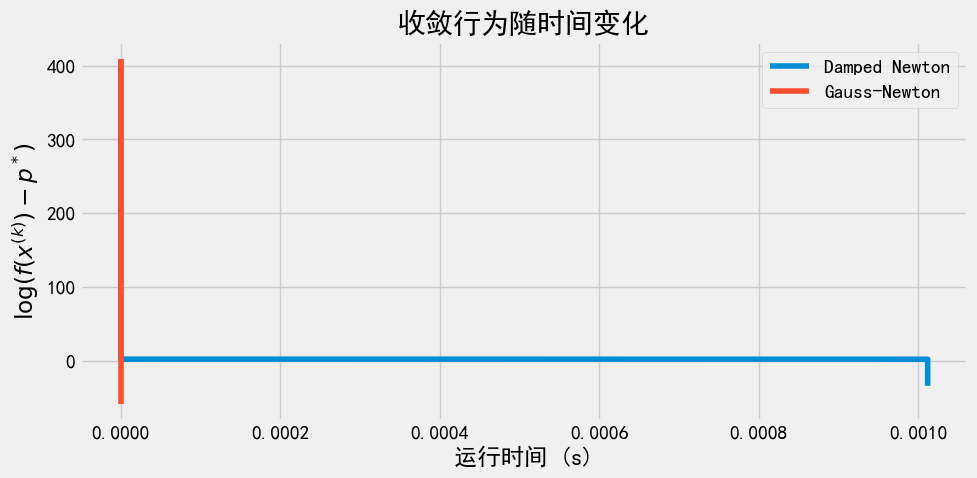
\includegraphics[width=\linewidth]{5-2.png}
        \caption{收敛行为随时间变化}\label{5-2}
    \end{minipage}
\end{figure}

\end{sol}

\question

\begin{sol}

根据Conjugate Direction方法,有$\bm{d}^{(k+1)} = -\bm{g}^{(k+1)} + \beta_k \bm{d}^{(k)}, k\ge 1$,所以根据共轭方向的性质$\bm{d}^{(k)}\bm{Q}\bm{d}^{(k-1)}=0$能够得到
\[\bm{d}^{(k)}\bm{Q}\bm{d}^{(k)} = -\bm{d}^{(k)}\bm{Q}\bm{g}^{(k)} + \beta_k \bm{d}^{(k)}\bm{Q}\bm{d}^{(k-1)} =  -\bm{d}^{(k)}\bm{Q}\bm{g}^{(k)}, k\ge 1.\]

当$k=0$时,由$\bm{d}^{(0)} = -\bm{g}^{(0)}$,$\bm{d}^{(0)}\bm{Q}\bm{d}^{(0)} = -\bm{d}^{(0)}\bm{Q}\bm{g}^{(0)}$。因此对$\forall k, \bm{d}^{(k)}\bm{Q}\bm{d}^{(k)} =-\bm{d}^{(k)}\bm{Q}\bm{g}^{(k)}$。

\end{sol}

\question 

\begin{sol}
  根据\textit{Opt\_book.pdf}中引理146,我们有  
\begin{equation}\label{lemma}
    \mathbf{g}^{(k+1)^T} \mathbf{d}^{(j)} = 0,\quad j = 0, 1, \dots, k.
\end{equation}

根据算法,对$1\le j\le k-1$
\[\mathbf{d}^{(j)} = -\mathbf{g}^{(j)} + \beta_{j-1} \mathbf{d}^{(j-1)},\]
所以
\[0 = \mathbf{g}^{(k+1)^T} \mathbf{d}^{(j)}  = -\mathbf{g}^{(k+1)^T} \mathbf{g}^{(j)} + \beta_{j-1} \mathbf{g}^{(k+1)^T} \mathbf{d}^{(j-1)}.\]
由于 $\mathbf{g}^{(k+1)^T} \mathbf{d}^{(j-1)} = 0$,有
\[\mathbf{g}^{(k+1)^T} \mathbf{g}^{(j)} = 0, 1\le j\le k-1.\]

$j = 0$时,$\mathbf{d}^{(0)} = -\mathbf{g}^{(0)}$, 所以$\mathbf{g}^{(k+1)^T} \mathbf{g}^{(0)} = -\mathbf{g}^{(k+1)^T} \mathbf{d}^{(0)} = 0$也成立。

\end{sol}

\question 

\begin{sol}

Backtracking参数$\alpha = 0.3, \beta = 0.5$,最多搜索$20$次;共轭梯度法的停止标准是$\nabla f(x)\le 10^{-6}$,最大迭代次数$20000$次。

我们测试了函数中的$\alpha\in[1,100,10000]$三种情况下三种$\beta$方法的表现。总体来讲FR方法初期下降最快,但接近目标值时速度放缓,HS方法恰恰相反,初期下降较慢,但最终收敛最快,PR中期较慢,其他时期介于两者之间。$\alpha$的变化影响目标函数的条件数,相对来讲$\alpha$越大问题条件数越差,收敛速度也就越慢。

\begin{table}[h]
\centering
\caption{不同 $\alpha$ 和 $\beta$ 方法组合下的共轭梯度法结果对比}
\resizebox{0.35\linewidth}{!}{
\begin{tabular}{cccccc}
\toprule
$\alpha$ & $\beta$ 方法 & 迭代次数 & 最终梯度范数 & 耗时 (s) & 最终函数值 \\
\midrule
\multirow{3}{*}{10000} 
& FR & 157 & $5.03 \times 10^{-7}$ & 0.1632 & $2.54 \times 10^{-13}$ \\
& PR & 130 & $2.94 \times 10^{-7}$ & 0.1388 & $1.90 \times 10^{-16}$ \\
& HS & 68  & $6.67 \times 10^{-7}$ & 0.0711 & $8.09 \times 10^{-17}$ \\
\midrule
\multirow{3}{*}{100} 
& FR & 137 & $8.37 \times 10^{-7}$ & 0.1199 & $7.34 \times 10^{-13}$ \\
& PR & 58  & $1.85 \times 10^{-7}$ & 0.0525 & $3.37 \times 10^{-14}$ \\
& HS & 33  & $7.78 \times 10^{-8}$ & 0.0256 & $2.12 \times 10^{-16}$ \\
\midrule
\multirow{3}{*}{1} 
& FR & 34  & $6.93 \times 10^{-7}$ & 0.0302 & $6.95 \times 10^{-13}$ \\
& PR & 31  & $6.82 \times 10^{-7}$ & 0.0234 & $3.63 \times 10^{-14}$ \\
& HS & 30  & $4.10 \times 10^{-7}$ & 0.0231 & $7.85 \times 10^{-14}$ \\
\bottomrule
\end{tabular}
}
\end{table}


\begin{figure}[h]
    \centering
    % 第一行:两张图
    \subfloat[$\alpha=10000$ 时的收敛行为]{
        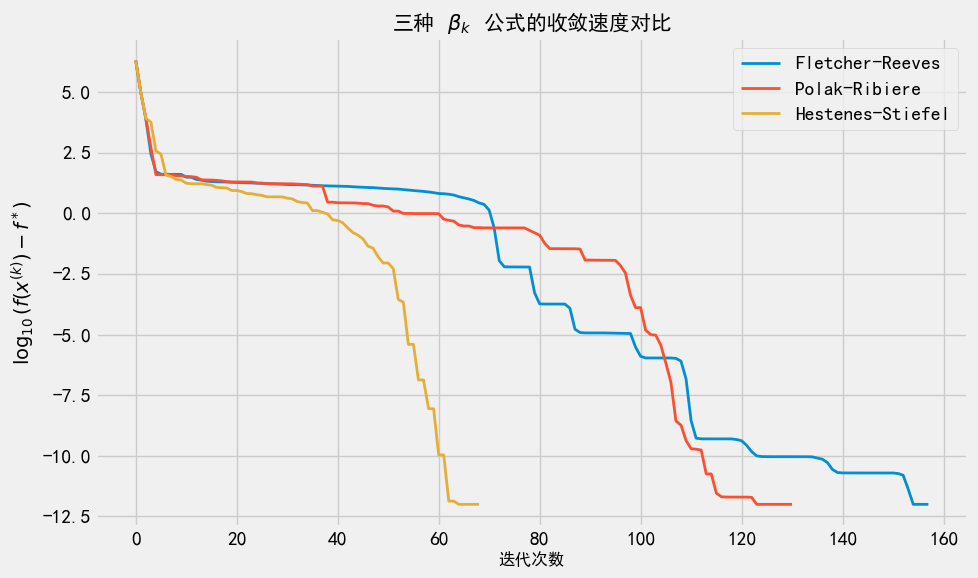
\includegraphics[width=0.6\linewidth]{8-1.png}
    }
    \vspace{1em}
    \subfloat[$\alpha=100$ 时的收敛行为]{
        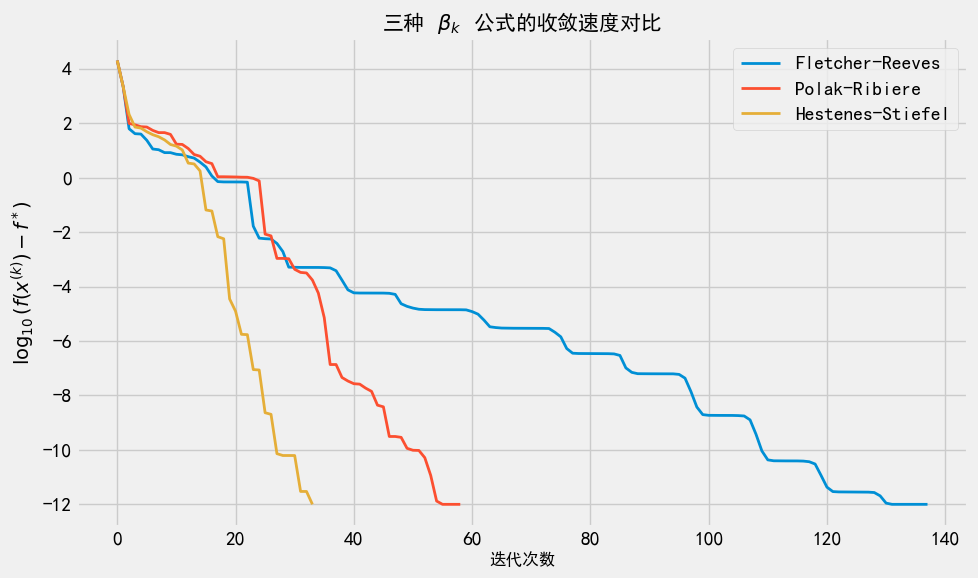
\includegraphics[width=0.6\linewidth]{8-2.png}
    }
    \vspace{1em}
    % 第二行:一张图
    \subfloat[$\alpha=1$ 时的收敛行为]{
        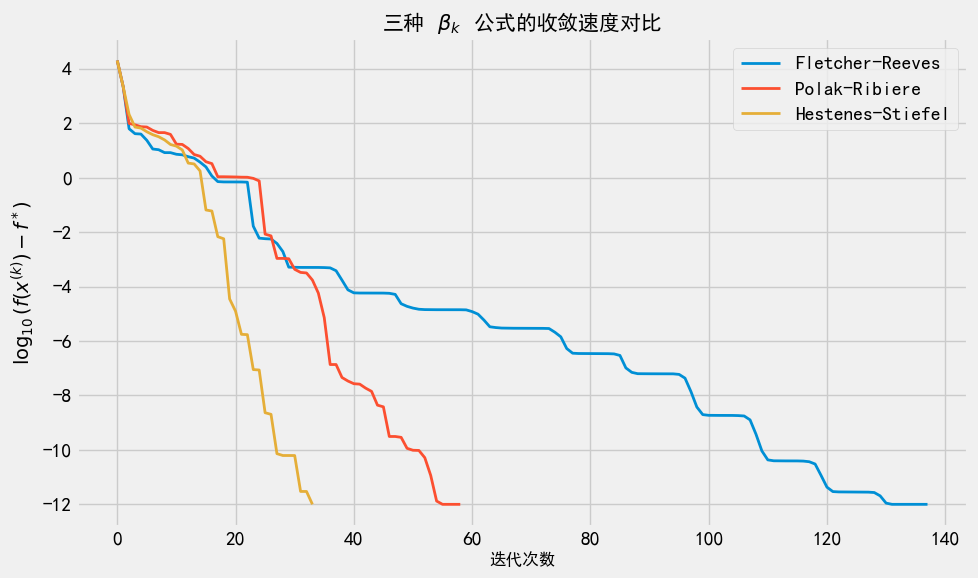
\includegraphics[width=0.6\linewidth]{8-3.png}
    }
    \caption{共轭梯度法在不同 $\alpha$ 下的收敛行为对比}
\end{figure}


\end{sol}

% citations
% \bibliographystyle{plain}
% \bibliography{citations}

\end{document}
